\documentclass[a4paper, 12pt]{article}

\def\languages{french, english}

%%%%%%%%%%%%%%%%%%% Libraries

%%%%%%%%%% Packages

%%%%% Coding tools

\usepackage{comment}
\usepackage{xstring}

%%%%% Encoding

\usepackage[utf8]{inputenc}
\usepackage[T1]{fontenc}
\usepackage{eurosym}

%%%%% Languages

\ifx\languages\undefined
	\usepackage[english]{babel}
\else
	\usepackage[\languages]{babel}
\fi

\def\languagefile{./include/languages/\languagename.tex}
\InputIfFileExists{\languagefile}{}

%%%%% Style

\usepackage{geometry}
\usepackage{fancyhdr}
\usepackage[bottom]{footmisc}

\edef\restoreparindent{\parindent=\the\parindent\relax}
\usepackage[parfill]{parskip}

\usepackage{enumitem}
\usepackage{csquotes}
\usepackage{color}

%%%%% Others

\usepackage[framemethod=TikZ]{mdframed}
\usepackage[pdfusetitle]{hyperref}

%%%%%%%%%% Features

%%%%% Settings

\geometry{paper=a4paper,top=3.5cm,bottom=2.5cm,right=2.5cm,left=2.5cm}

\pagestyle{fancy}
\fancyhead[L]{}
\fancyhead[R]{\leftmark}
\fancyfoot[C]{\thepage}
\renewcommand{\headrulewidth}{0pt}

%\restoreparindent

%%%%% Commands

\newcommand{\romantableofcontents}{
	\newpage
	\pagenumbering{roman}
	\tableofcontents
	\newpage
	\pagenumbering{arabic}
}

%%%%%%%%%% Packages

\usepackage{float}
\usepackage[skip=1em]{caption}

\usepackage{array}
\usepackage{multirow}
\usepackage{multicol}

%%%%%%%%%% Features

%%%%% Settings

\renewcommand{\arraystretch}{1.2}

%%%%% Commands

\newcommand\noskipcaption[1]{\caption{#1}\vspace{-1em}}

%%%%%%%%%% Packages

\usepackage{inconsolata}
\usepackage{listings}

%%%%%%%%%% Features

%%%%% Commands

\newcommand{\Nstyle}[1]{
    \lstdefinestyle{N#1}{
        style=#1,
        %%%%%
        numbers=left
    }
}

\newcommand{\tbFstyle}[1]{
    \lstdefinestyle{tbF#1}{
        style=#1,
        %%%%%
        frame=tb
    }
}

\newcommand{\Fstyle}[1]{
    \lstdefinestyle{F#1}{
        style=#1,
        %%%%%
        frame=single,
        framesep=0em,
        rulesep=0em,
        xleftmargin=0.75em,
        xrightmargin=0.75em,
        framexleftmargin=0.75em,
        framexrightmargin=0.75em,
        framextopmargin=0.5em,
        framexbottommargin=0.5em,
        %%%%%
        numbersep=1.25em
    }
}

\newcommand{\NtbFstyle}[1]{
    \tbFstyle{#1}
    \Nstyle{tbF#1}
}

\newcommand{\NFstyle}[1]{
    \Fstyle{#1}
    \lstdefinestyle{NF#1}{
        style=f#1,
        %%%%%
        xleftmargin=2.75em,
        framexleftmargin=2.75em,
        %%%%%
        numbers=left,
        numbersep=1em
    }
}

%%%%% Styles

\lstdefinestyle{default}{
    breaklines=true,
    breakatwhitespace=true,
    columns=fixed,
	extendedchars=true,
    upquote=true,
	tabsize=4,
    %%%%%
    framerule=0.66pt,
    captionpos=b,
	%%%%%
    basicstyle=\footnotesize\ttfamily,
    numberstyle=\footnotesize\ttfamily,
    showstringspaces=false
}
\Nstyle{default}
\NFstyle{default}
\NtbFstyle{default}

\lstdefinestyle{monokai}{
    style=Fdefault,
    %%%%%
    backgroundcolor=\color[HTML]{272822},
    framerule=0em,
    %%%%%
    basicstyle=\footnotesize\ttfamily\color[HTML]{f8f8f2},
    numberstyle=\footnotesize\ttfamily\color[HTML]{272822},
    commentstyle=\color[HTML]{75715e},
    keywordstyle=[1]{\color[HTML]{f92672}},
    keywordstyle=[2]{\color[HTML]{A6E22E}},
    keywordstyle=[3]{\color[HTML]{ae81ff}},
    stringstyle=\color[HTML]{e6db74},
    %%%%%
    % otherkeywords={!,.,+,-,*,/,=,<,>,^,|,\&,OR,AND}
}

\lstdefinestyle{Nmonokai}{
    style=monokai,
    %%%%%
    xleftmargin=2.75em,
    framexleftmargin=2.75em,
    %%%%%
    numbers=left,
    numberstyle=\footnotesize\ttfamily\color[HTML]{f8f8f2},
    numbersep=1em
}

\lstdefinestyle{c}{
    language=C,
    style=default,
    %%%%%
    commentstyle=\color[HTML]{228B22},
    keywordstyle=\color[HTML]{0000FF},
    stringstyle=\color[HTML]{A020F0},
    emphstyle=\color[HTML]{0000FF},
    %%%%%
    emph={}
}

\lstdefinestyle{cpp}{
    language=C++,
    style=default,
    %%%%%
    commentstyle=\color[HTML]{228B22},
    keywordstyle=\color[HTML]{0000FF},
    stringstyle=\color[HTML]{A020F0},
    emphstyle=\color[HTML]{0000FF},
    %%%%%
    emph={std}
}

\lstdefinestyle{matlab}{
    language=matlab,
    style=default,
    %%%%%
    basicstyle=\footnotesize\fontfamily{pcr}\selectfont,
    numberstyle=\footnotesize\fontfamily{pcr}\selectfont,
    commentstyle=\color[HTML]{228B22},
    keywordstyle=\color[HTML]{0000FF},
    stringstyle=\color[HTML]{A020F0},
    emphstyle=\color[HTML]{0000FF},
    %%%%%
    emph={clearvars}
}

\lstdefinestyle{python}{
    language=python,
    style=default,
    %%%%%
    commentstyle=\color[RGB]{221,0,0},
    keywordstyle=[1]{\color[RGB]{255,119,0}},
    keywordstyle=[2]{\color[RGB]{144,0,144}},
    stringstyle=\color[RGB]{0,170,0},
    emphstyle=\color[RGB]{255,119,0},
    %%%%%
    emph={}
}

\lstdefinestyle{java}{
    language=java,
    style=default,
    %%%%%
    commentstyle=\color[HTML]{228B22},
    keywordstyle=\color[HTML]{0000FF},
    stringstyle=\color[HTML]{A020F0},
    emphstyle=\color[HTML]{0000FF},
    %%%%%
    emph={}
}

%%%%%%%%%% Packages

\usepackage{amsmath}
\usepackage{amssymb}
\usepackage{bm}
\usepackage{esint}
\usepackage[makeroom]{cancel}

%%%%%%%%%% Features

%%%%% Macros

\newcommand{\rbk}[1]{\left(#1\right)}
\newcommand{\cbk}[1]{\left\{#1\right\}}
\newcommand{\sbk}[1]{\left[#1\right]}
\newcommand{\abs}[1]{\left|#1\right|}
\newcommand{\norm}[1]{\left\|#1\right\|}

\newcommand{\fact}[1]{#1!}
\newcommand{\e}[1]{\mathbf{e}_{#1}}
\newcommand{\deriv}{\mathrm{d}}
\DeclareMathOperator{\tr}{tr}

\def\Rl{\mathbb{R}}
\def\Cx{\mathbb{C}}
\def\Na{\mathbb{N}}
\def\Zi{\mathbb{Z}}

%%%%%%%%%% Packages

\usepackage{amsthm}
\usepackage{thmtools}

%%%%%%%%%% Features

%%%%% Settings

\makeatletter
\define@key{thmdef}{mdthm}[{}]{
	\thmt@trytwice{\def\thmt@theoremdefiner{\mdtheorem[#1]}}{}}
\makeatother

\begingroup
\makeatletter
\@for\theoremstyle:=plain,definition,remark\do{
	\expandafter\g@addto@macro\csname th@\theoremstyle\endcsname{
		\addtolength\thm@preskip\parskip
	}
}
\endgroup

\renewcommand{\qedsymbol}{$\blacksquare$}

% language

\ifx\lgthm\undefined
	\def\lgthm{Theorem}
	\def\lgprf{Proof}
	\def\lglem{Lemma}
	\def\lgprop{Proposition}
	\def\lgdefn{Definition}
	\def\lghyp{Hypothesis}
	\def\lgmeth{Method}
	\def\lgquest{Question}
	\def\lgansw{Answer}
	\def\lgexpl{Example}
	\def\lgrmk{Remark}
	\def\lgnote{Note}
	\def\lgtip{Tip}
\fi

%%%%% Commands

\newcommand\qedadd{\pushQED{\qed}\popQED}

%%%%% Environments

\theoremstyle{plain}
\newtheorem{thm}{\lgthm}
\newtheorem{lem}[thm]{\lglem}
\newtheorem{prop}[thm]{\lgprop}

\theoremstyle{definition}
\newtheorem{defn}{\lgdefn}
\newtheorem{hyp}{\lghyp}
\newtheorem{meth}{\lgmeth}
\newtheorem{quest}{\lgquest}

\theoremstyle{remark}
\newtheorem{answ}{\lgansw}[quest]
\newtheorem{expl}{\lgexpl}
\newtheorem*{rmk}{\lgrmk}
\newtheorem*{note}{\lgnote}
\newtheorem*{tip}{\lgtip}

% framed

\mdfdefinestyle{thicc}{
	nobreak=true,
	skipabove=\topskip,
	skipbelow=\topskip,
	innerleftmargin=0.5em,
	innerrightmargin=0.5em,
	innerbottommargin=0.5em,
	innertopmargin=0.5em,
	linewidth=0.25em,
	roundcorner=0.15em,
	linecolor=black!10,
	frametitlebackgroundcolor=black!10,
	theoremseparator={.}
}

\declaretheorem[mdthm={style=thicc, linecolor=red!20, frametitlebackgroundcolor=red!20}, sibling=thm, name=\lgthm]{framedthm}
\declaretheorem[mdthm={style=thicc, linecolor=red!20, frametitlebackgroundcolor=red!20}, sibling=thm, name=\lglem]{framedlem}
\declaretheorem[mdthm={style=thicc, linecolor=blue!20, frametitlebackgroundcolor=blue!20}, sibling=thm, name=\lgprop]{framedprop}
\declaretheorem[mdthm={style=thicc, nobreak=false}, parent=thm, name=\lgprf]{framedprf}

\declaretheorem[mdthm={style=thicc, linecolor=black!20!green!20, frametitlebackgroundcolor=black!20!green!20}, sibling=defn, name=\lgdefn]{frameddefn}
\declaretheorem[mdthm={style=thicc, linecolor=blue!20, frametitlebackgroundcolor=blue!20}, sibling=hyp, name=\lghyp]{framedhyp}
\declaretheorem[mdthm={style=thicc}, name=\lgmeth]{framedmeth}
\declaretheorem[mdthm={style=thicc, linecolor=orange!20, frametitlebackgroundcolor=orange!20}, sibling=quest, name=\lgquest]{framedquest}

\declaretheorem[mdthm={style=thicc, nobreak=false}, sibling=answ, name=\lgansw]{framedansw}
\declaretheorem[mdthm={style=thicc, nobreak=false}, sibling=expl, name=\lgexpl]{framedexpl}

%%%%%%%%%% Packages

\usepackage{siunitx}

%%%%%%%%%% Features

%%%%% Settings

\ifx\decimalsign\undefined
\else
    \sisetup{output-decimal-marker = \decimalsign}
\fi


%%%%% Settings

% lists
\frenchbsetup{StandardLists=true}

% units
\def\decimalsign{,}

% captions
\addto\captionsfrench{\def\figurename{Figure}}
\addto\captionsfrench{\def\tablename{Table}}
\addto\captionsfrench{\def\proofname{Preuve}}

% theorems

\def\lgthm{Théorème}
\def\lgprf{Preuve}
\def\lglem{Lemme}
\def\lgprop{Proposition}
\def\lgdefn{Définition}
\def\lghyp{Hypothèse}
\def\lgmeth{Méthode}
\def\lgquest{Question}
\def\lgansw{Réponse}
\def\lgexpl{Exemple}
\def\lgrmk{Remarque}
\def\lgnote{Note}
\def\lgtip{Conseil}

%%%%% Macros

\def\tq{\text{t.q.}}
\def\cad{c.-à-d.}
\def\Cad{C.-à-d.}


%%%%%%%%%%%%%%%%%%% Titlepage

\def\logopath{resources/pdf/logo-uliege.pdf}
\def\toptitle{University of Liège}
\title{Homework 1}
\def\subtitle{Applied digital signal processing}
%\def\authorhead{Author}
\author{
    Quentin \textsc{Graillet} (20164386)\\
    Maxime \textsc{Meurisse} (20161278)\\
    Adrien \textsc{Schoffeniels} (20162843)\\
}
%\def\rightauthorhead{}
%\def\rightauthor{}
\def\context{3\ieme{} year of Bachelor Civil Engineer}
\date{Academic year 2018-2019}

%%%%%%%%%%%%%%%%%%% Others

\NFstyle{matlab}

%%%%%%%%%%%%%%%%%%% Document

\begin{document}
	%%%%%%%%%% Packages

%%%%% Coding tools

\usepackage{comment}
\usepackage{xstring}

%%%%% Encoding

\usepackage[utf8]{inputenc}
\usepackage[T1]{fontenc}
\usepackage{eurosym}

%%%%% Languages

\ifx\languages\undefined
	\usepackage[english]{babel}
\else
	\usepackage[\languages]{babel}
\fi

\def\languagefile{./include/languages/\languagename.tex}
\InputIfFileExists{\languagefile}{}

%%%%% Style

\usepackage{geometry}
\usepackage{fancyhdr}
\usepackage[bottom]{footmisc}

\edef\restoreparindent{\parindent=\the\parindent\relax}
\usepackage[parfill]{parskip}

\usepackage{enumitem}
\usepackage{csquotes}
\usepackage{color}

%%%%% Others

\usepackage[framemethod=TikZ]{mdframed}
\usepackage[pdfusetitle]{hyperref}

%%%%%%%%%% Features

%%%%% Settings

\geometry{paper=a4paper,top=3.5cm,bottom=2.5cm,right=2.5cm,left=2.5cm}

\pagestyle{fancy}
\fancyhead[L]{}
\fancyhead[R]{\leftmark}
\fancyfoot[C]{\thepage}
\renewcommand{\headrulewidth}{0pt}

%\restoreparindent

%%%%% Commands

\newcommand{\romantableofcontents}{
	\newpage
	\pagenumbering{roman}
	\tableofcontents
	\newpage
	\pagenumbering{arabic}
}

	\section{Magnitude response of a filter}
	We consider a filter with the transfer function
	\begin{equation*}
	    H(z) = \dfrac{b_0}{\sbk{1-2r\cos\rbk{\omega_0}z^{-1}+r^2z^{-2}}^K}
	\end{equation*}
	To simplify the study of this function, we consider that it is a cascade of K second-order filters. The function can therefore be decomposed into a product of elementary transfer functions.
	\begin{equation*}
	    H(z) = K\rbk{\dfrac{b_0^{\frac{1}{K}}}{1-2r\cos\rbk{\omega_0}z^{-1}+r^2z^{-2}}}
	\end{equation*}
	We replace the parameters $K$, $r$ and $b_0$ by their value, and we store the coefficients of the numerator in a vector $b$, and those of the denominator in a vector $a$. We define a linearly spaced vector ranging from $-\pi$ to $\pi$ and having \num{500} points. We then use the function \texttt{freqz} of Matlab\footnote{All Matlab codes used are attached to this report.} with these data and we display the result.\par
	The magnitude response for $\omega_0 = \frac{\pi}{3}$ is shown in figure \ref{fig:magnitude_response_a}. To obtain the values of the magnitude in \deci\bel, we multiply all the values $x$ by $10\log_{10}(x)$. The normalized angular frequency is scaled by $\pi$.\par
	\begin{figure}[!ht]
	    \centering
	    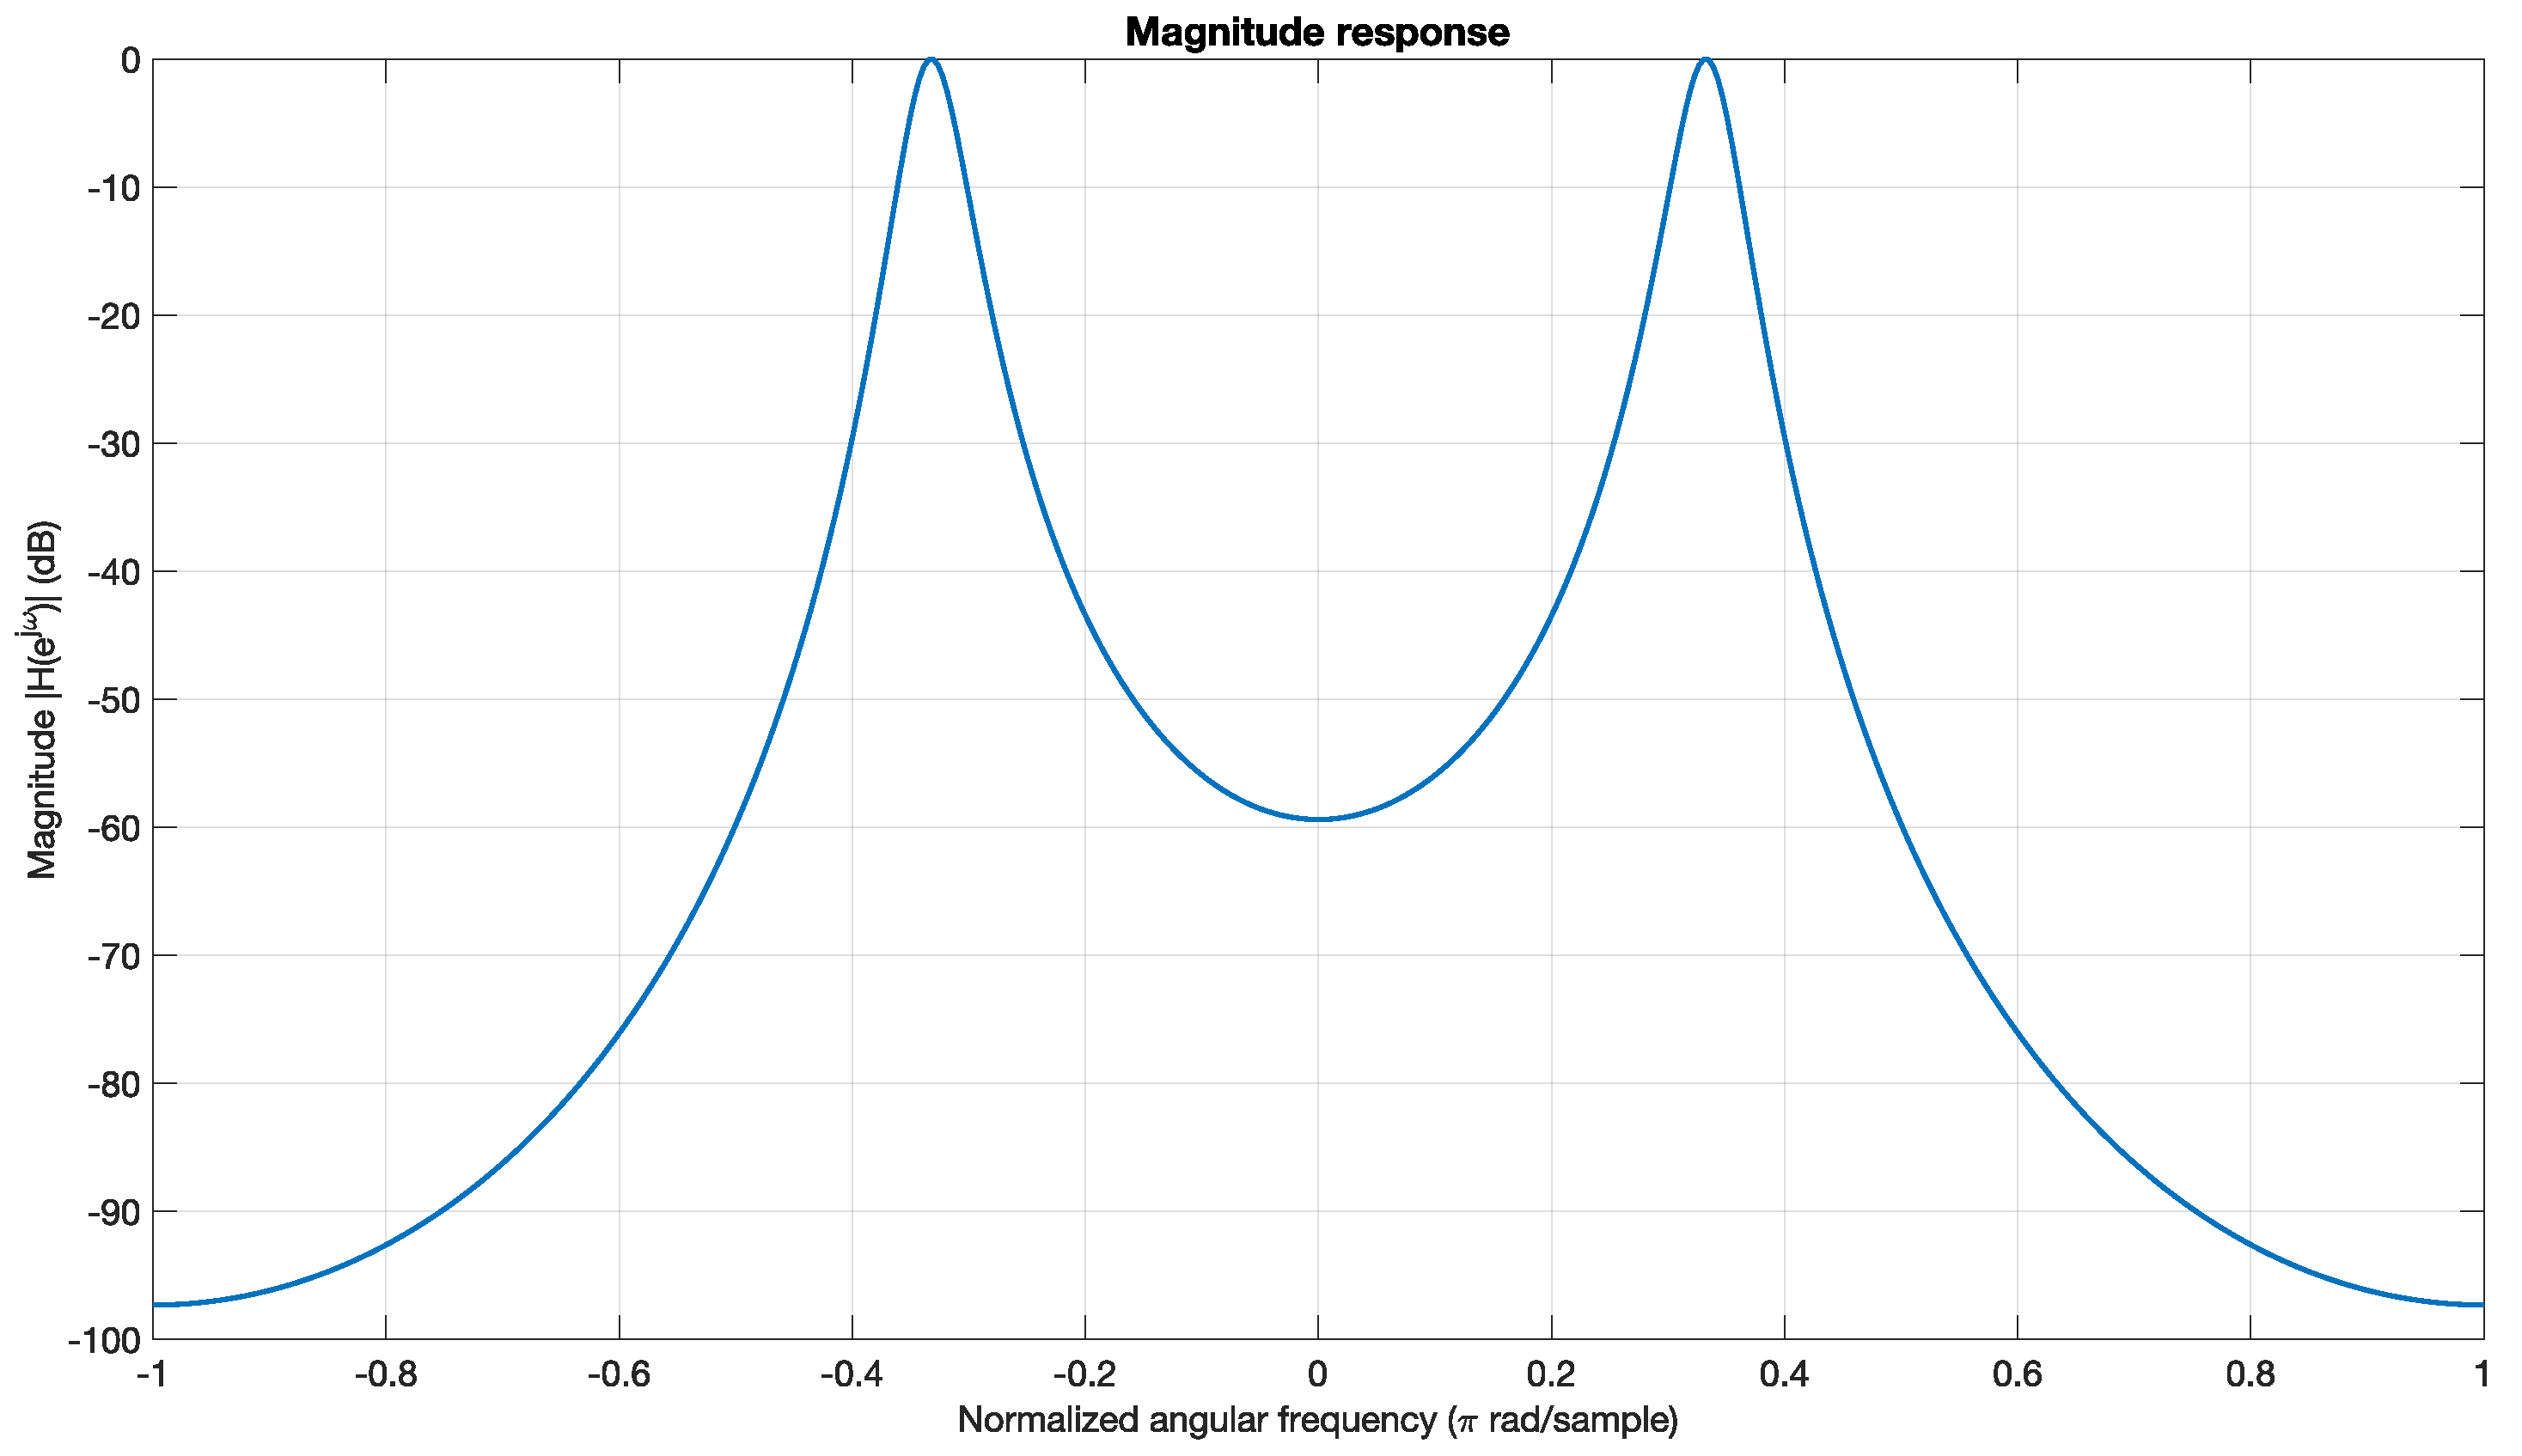
\includegraphics[width=1\textwidth]{resources/pdf/magnitude_response_a.pdf}
	    \caption{Magnitude response $\abs{H(e^{j\omega})}$ for $\omega_0 = \frac{\pi}{3}$.}
	    \label{fig:magnitude_response_a}
	\end{figure}
	We repeat the same procedure for $\omega = \frac{2\pi}{3}$ (figure \ref{fig:magnitude_response_b}).\par
	\begin{figure}[!ht]
	    \centering
	    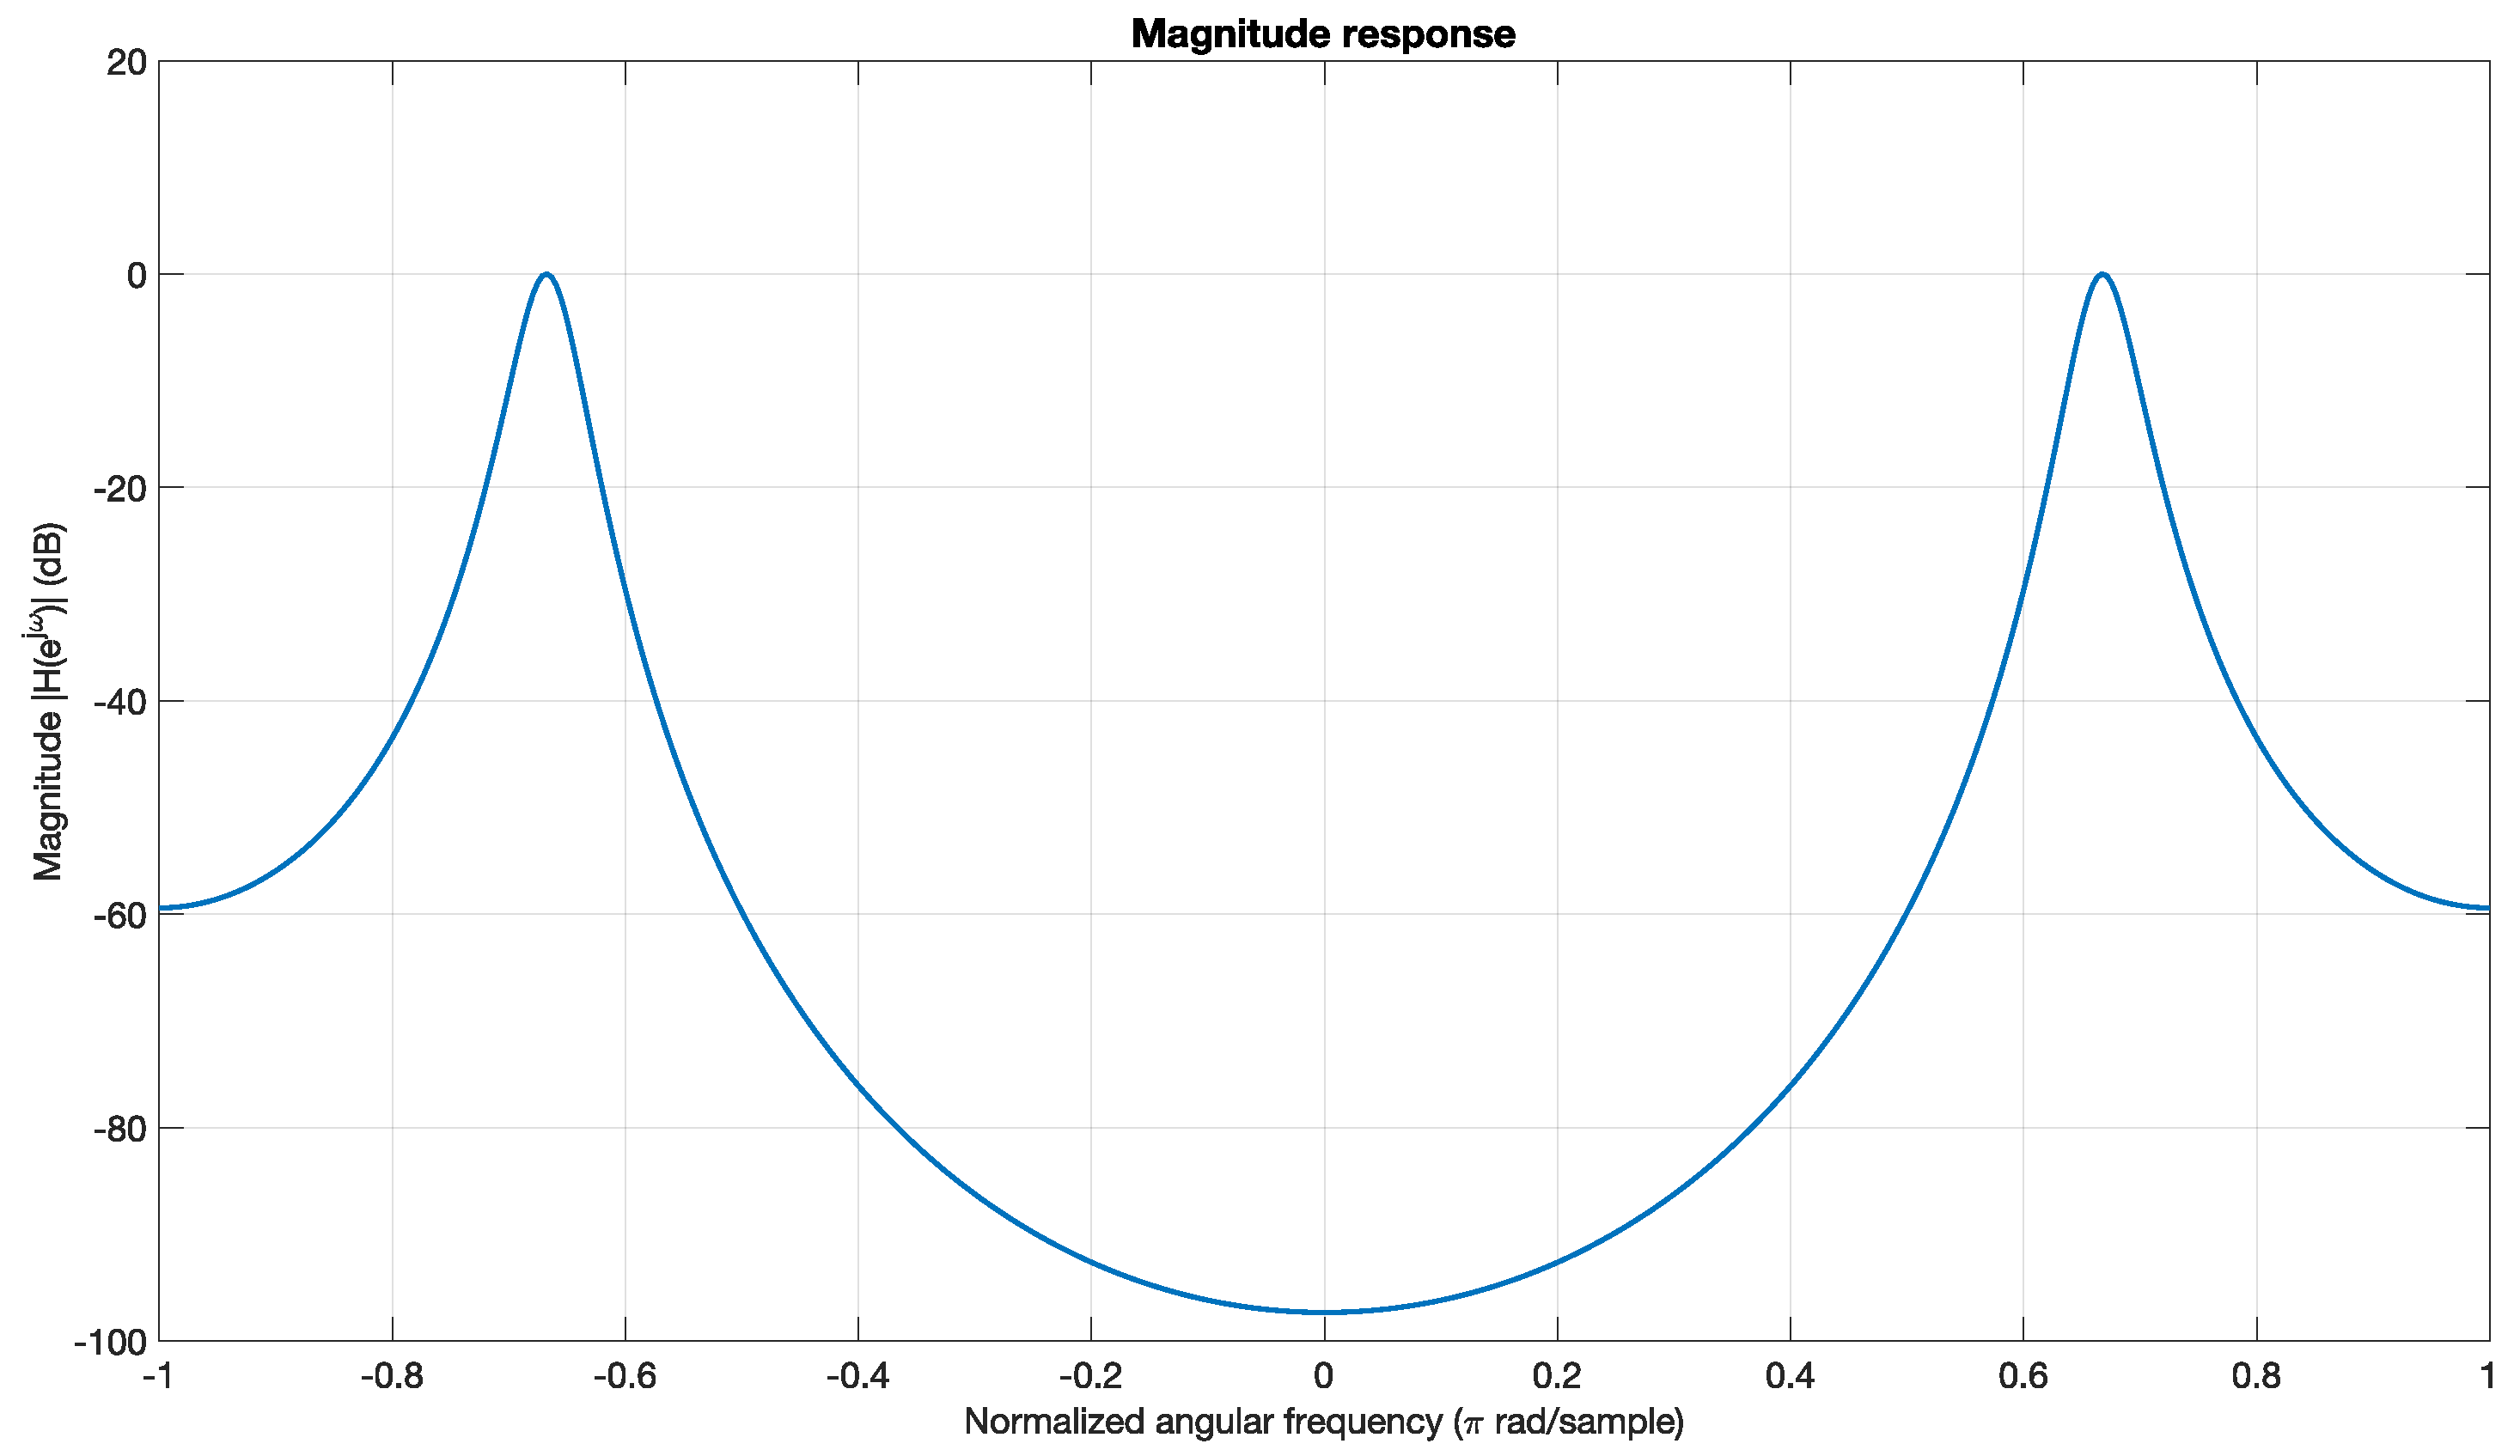
\includegraphics[width=1\textwidth]{resources/pdf/magnitude_response_b.pdf}
	    \caption{Magnitude response $\abs{H(e^{j\omega})}$ for $\omega_0 = \frac{2\pi}{3}$.}
	    \label{fig:magnitude_response_b}
	\end{figure}
	Examining figures \ref{fig:magnitude_response_a} and \ref{fig:magnitude_response_b}, we found that it is a band-pass filter. Indeed, this filter passes only a frequency band around the value $\omega_0$.\par
	By varying the value of this parameter $\omega_0$, we observe that the band-pass filter does not let the same frequency band pass.\par
	In conclusion, the impact of the change of the parameter $\omega_0$ is implicit. This defines which frequency band the filter will pass.
	\newpage
	\section{Autocorrelation of a single echo}
	Let the expression of a single echo $y[n]$ generated using the FIR filter
	\begin{equation}
	    \label{eq:echo_y}
	    \tag{$\dagger$}
	    y[n] = x[n] + ax[n-D],\quad -1<a<1
	\end{equation}
	By definition, the expression of the autocorrelation $r_y[l]$ is given by
	\begin{equation*}
	    r_y[l] = \sum_{n=-\infty}^{\infty}y[n]\times y[n-l]
	\end{equation*}
	We can replace $y[n]$ by its expression \eqref{eq:echo_y}
	\begin{equation*}
	    r_y[l] = \sum_{n=-\infty}^{\infty}(x[n]+ax[n-D])\times (x[n-l] + ax[n-l-D])
	\end{equation*}
	By distributing, we get
	\begin{align*}
	    r_y[l] &= \sum_{n=-\infty}^{\infty}(a_1+a_2+a_3+a_4)\\
	    &= \sum_{n=-\infty}^{\infty}a_1 + \sum_{n=-\infty}^{\infty}a_2 + \sum_{n=-\infty}^{\infty}a_3 + \sum_{n=-\infty}^{\infty}a_4
	\end{align*}
	where
	\begin{itemize}
	    \item $a_1 = x[n]\times x[n-l]$
	    \item $a_2 = x[n]\times ax[n-l-D]$
	    \item $a_3 = ax[n-D]\times x[n-l] = ax[n-D]\times x[n-D-\rbk{l-D}]$
	    \item $a_4 = ax[n-D]\times ax[n-l-D]$
	\end{itemize}
	We note that we fall back on the definition of the autocorrelation of the signal $x$. By replacing the terms with this definition, we find the expression of the autocorrelation $r_y[l]$ in terms of the autocorrelation $r_x[l]$, $D$ and $a$
	\begin{align*}
	    r_y[l] &= r_x[l] + ar_x[l+D] + ar_x[l-D] + a^2r_x[l]\\
	    &= (1+a^2)r_x[l] + a\rbk{r_x[l-D] + r_x[l+D]}
	\end{align*}
	\newpage
	\section{Echo cancellation}
	Using the \texttt{audioread} and \texttt{xcorr} functions of Matlab, we play the sound and plot its autocorrelation function (figure \ref{fig:sound_autocorrelation}).\par
	\begin{figure}[!ht]
	    \centering
	    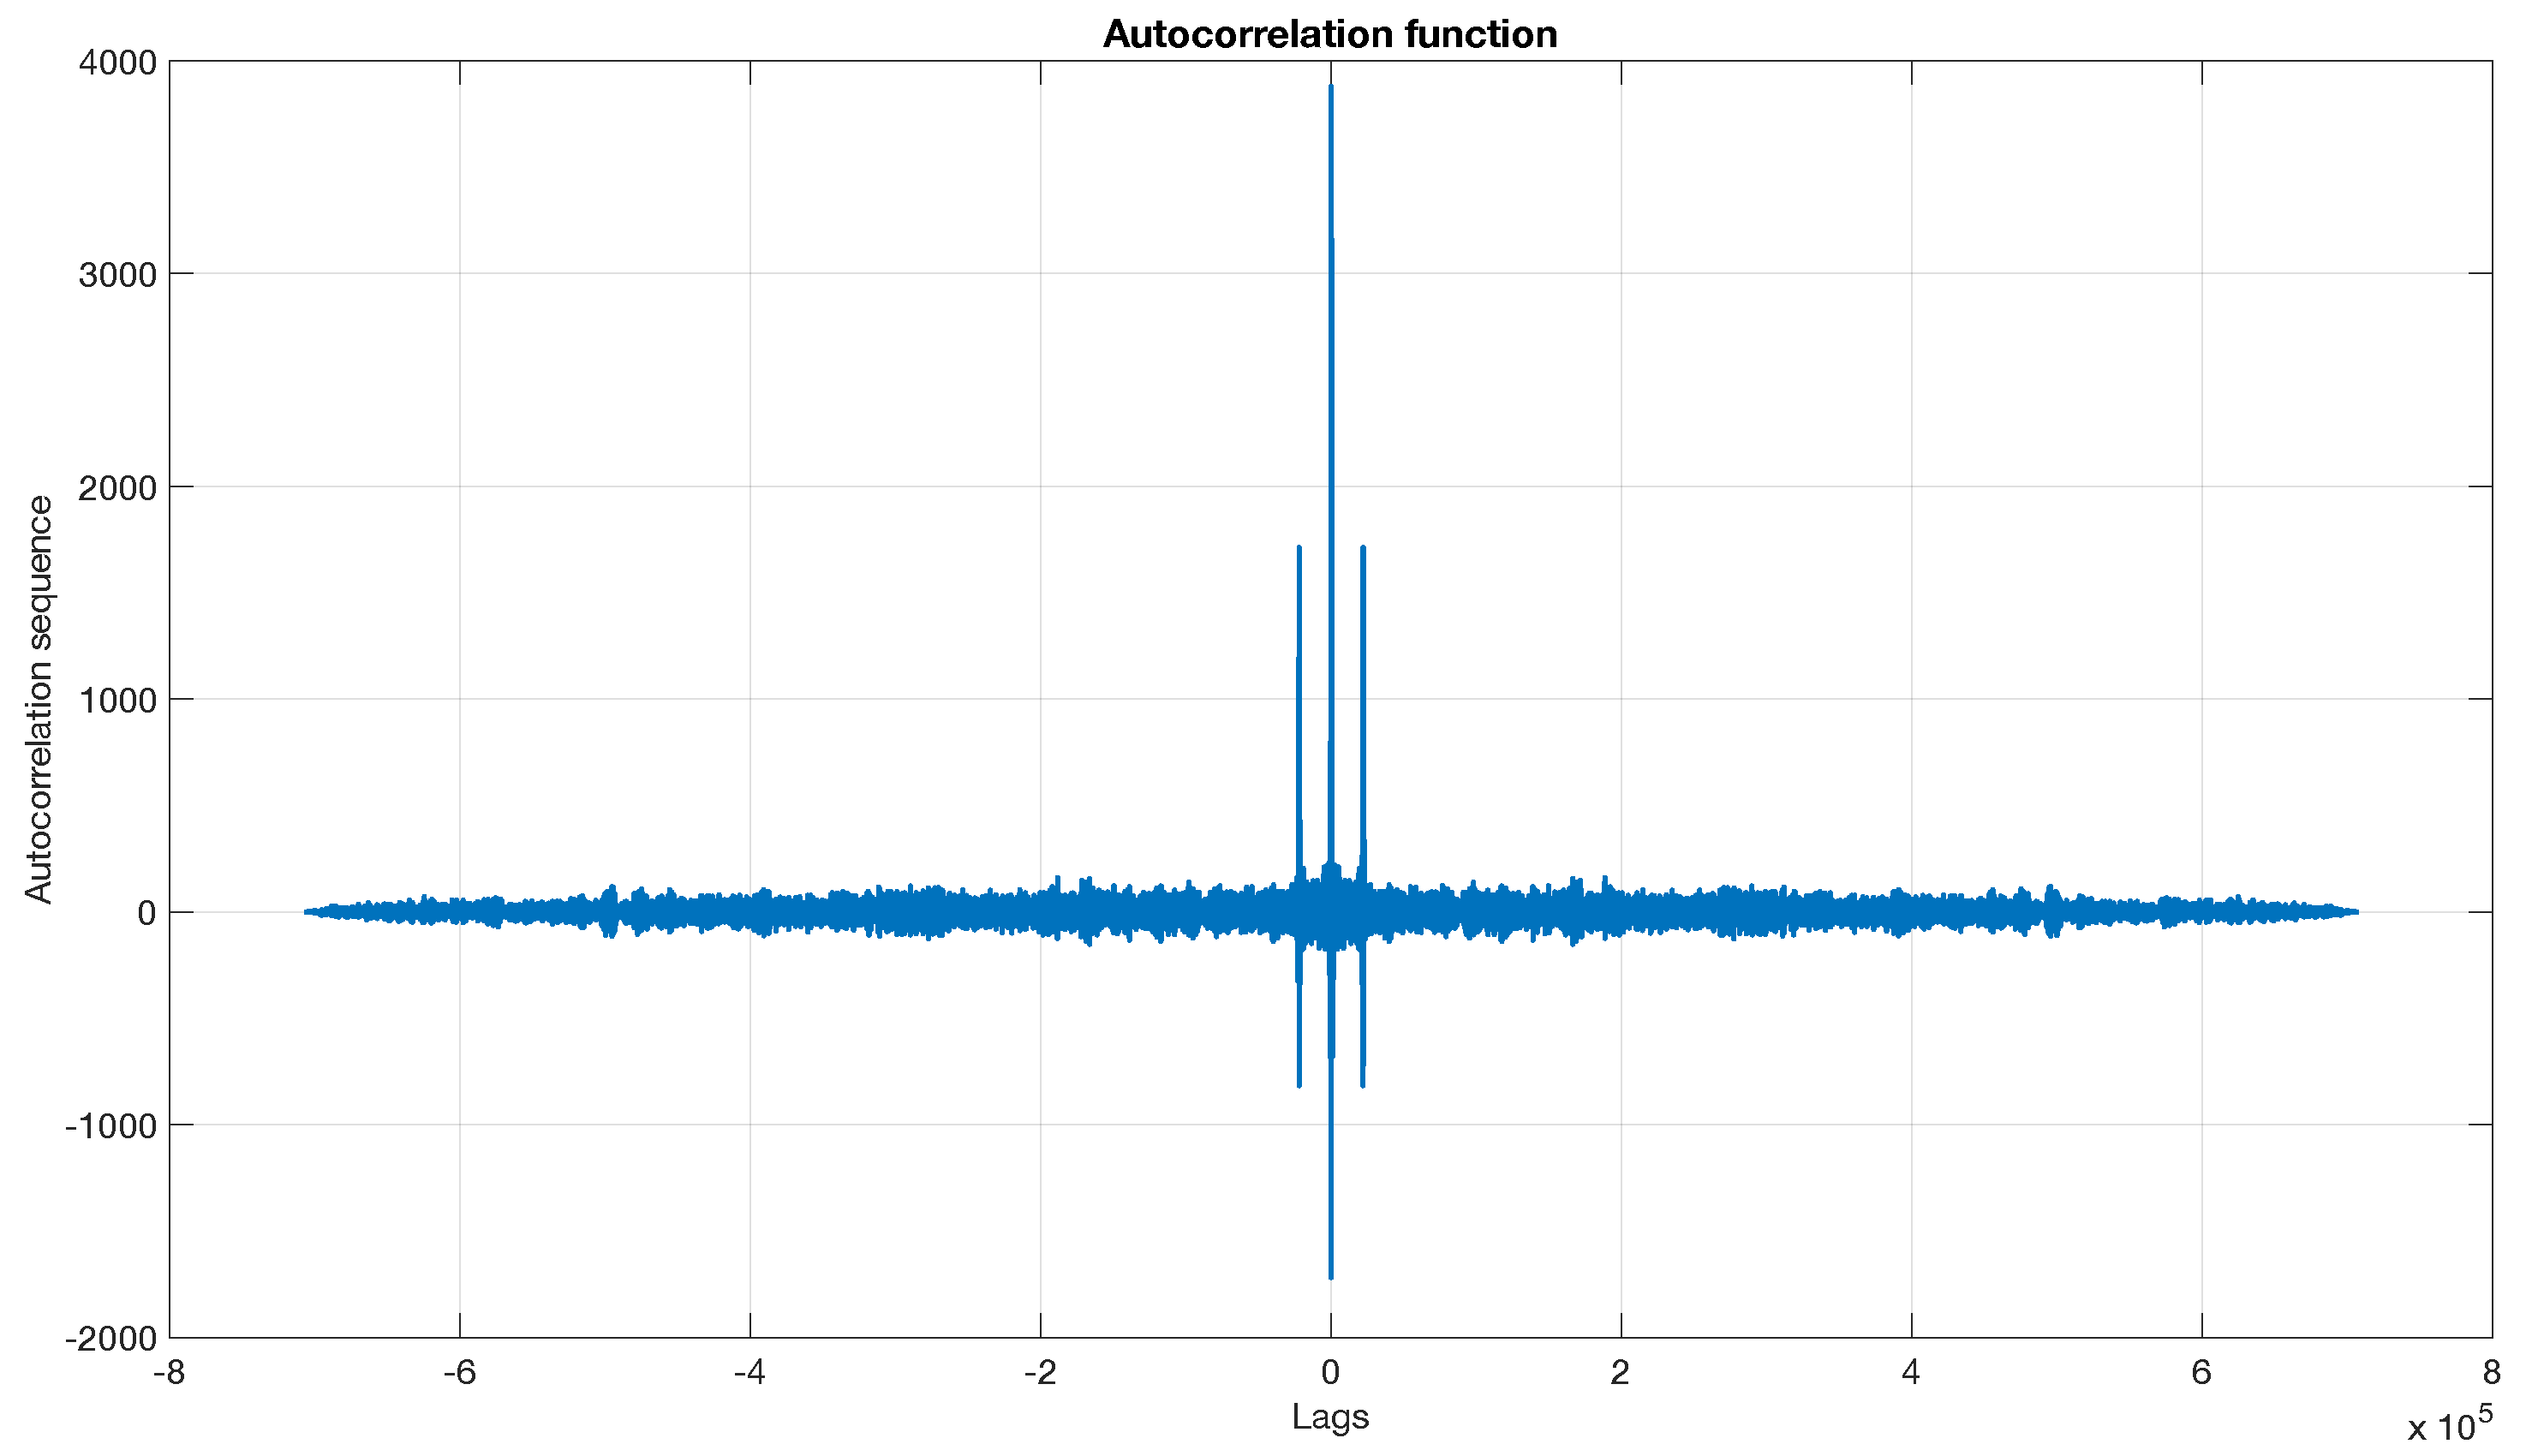
\includegraphics[width=1\textwidth]{resources/pdf/sound_autocorrelation.pdf}
	    \caption{Autocorrelation function of the sound \texttt{hw1\_echo.wav}.}
	    \label{fig:sound_autocorrelation}
	\end{figure}
	The expression of the signal with echo is given by
	\begin{equation*}
	    y(n) = x(n) + \alpha x(n-d)
	\end{equation*}
	with $x(n)$, the original sound without echo. The goal is to recover $x(n)$.\par
	By passing into the frequency domain, we have
	\begin{equation*}
	    Y(z) = X(z) + \alpha X(z)z^{-d}
	\end{equation*}
	We can find the transfer function
	\begin{align*}
	    H(z) &= \dfrac{Y(z)}{X(z)}\\
	    &= 1 + \alpha z^{-d}
	\end{align*}
	And so, we have
	\begin{equation*}
	    X(z) = \dfrac{Y(z)}{H(z)}
	\end{equation*}
	This means that we need to filter the observed signal $y(n)$ through the filter $\frac{1}{H(z)}$ in order to recover $x(n)$. To build the transfer function, we have to find the delay $d$.\par
	In the figure \ref{fig:sound_autocorrelation}, several peaks are observed. The delay can be found by observing the distance between two consecutive peaks.\par
	We thus find the delay (expressed in number of sampling intervals) $d = \num{2.205e4}$. We can also find the corresponding delay expressed in seconds by divising this value by \texttt{fs}. We obtain (in seconds): $\tau = \num{0.5}$.\par
	We assume that the amplitude of the reflected sound is sixty percent of the emitted one, so $\alpha = 0.6$. We can now build the coefficients of the transfer function. These are stored in the vectors $b$ (for the numerator) and $a$ (for the denominator).\par
	Now just call the function \texttt{filter} of Matlab with as arguments the vectors containing the coefficients and the sound to be filtered. The new sound obtained can be played with the function \texttt{sound} of Matlab. It can be seen that it no longer contains an echo.
	\newpage
	\appendix
	\section{Matlab codes}
	\subsection{Magnitude response of a filter}
	\lstinputlisting[style=NFmatlab]{resources/m/Q1.m}
	\subsection{Echo cancellation}
	\lstinputlisting[style=NFmatlab]{resources/m/Q3.m}
\end{document}
